\documentclass[12pt, a4paper]{article}
\usepackage{caption}
\usepackage{graphicx}
\usepackage{hyperref}
\hypersetup{
    colorlinks,
    citecolor=black,
    filecolor=black,
    linkcolor=black,
    urlcolor=black
} 

\usepackage{tikz-network}
\usepackage{amsmath, amsfonts, amssymb, amsthm}
\usepackage{algpseudocode}
\usepackage{algorithm}
\title{Computer Architecture\\and system programming}
\date{2022}
\author{Kristoffer Klokker}

\usepackage{xcolor,listings}
\usepackage{textcomp}
\usepackage{color}
\usepackage{listings}
\definecolor{codegreen}{rgb}{0,0.6,0}
\definecolor{codegray}{rgb}{0.5,0.5,0.5}
\definecolor{codepurple}{HTML}{C42043}
\definecolor{backcolour}{HTML}{F2F2F2}
\definecolor{bookColor}{cmyk}{0,0,0,0.90}  
\color{bookColor}

\lstset{upquote=true}

\lstdefinestyle{mystyle}{
    backgroundcolor=\color{backcolour},   
    commentstyle=\color{codegreen},
    keywordstyle=\color{codepurple},
    numberstyle=\numberstyle,
    stringstyle=\color{codepurple},
    basicstyle=\footnotesize\ttfamily,
    breakatwhitespace=false,
    breaklines=true,
    captionpos=b,
    keepspaces=true,
    numbers=left,
    numbersep=10pt,
    showspaces=false,
    showstringspaces=false,
    showtabs=false,
    tabsize=3,
}


\lstset{style=mystyle}
\usepackage{zref-base}

\makeatletter
\newcounter{mylstlisting}
\newcounter{mylstlines}
\lst@AddToHook{PreSet}{%
  \stepcounter{mylstlisting}%
  \ifnum\mylstlines=1\relax
    \lstset{numbers=none}
  \else
    \lstset{numbers=left}
  \fi
  \setcounter{mylstlines}{0}%
}
\lst@AddToHook{EveryPar}{%
  \stepcounter{mylstlines}%
}
\lst@AddToHook{ExitVars}{%
  \begingroup
    \zref@wrapper@immediate{%
      \zref@setcurrent{default}{\the\value{mylstlines}}%
      \zref@labelbyprops{mylstlines\the\value{mylstlisting}}{default}%
    }%
  \endgroup
}

% \mylstlines print number of lines inside listing caption
\newcommand*{\mylstlines}{%
  \zref@extractdefault{mylstlines\the\value{mylstlisting}}{default}{0}%
}
\makeatother


\newcommand\numberstyle[1]{%
    \footnotesize
    \color{codegray}%
    \ttfamily
    \ifnum#1<10 0\fi#1 |%
}


\begin{document}
	\maketitle
	\clearpage
	\tableofcontents
	\clearpage
	\section{Exercises}
		\subsection{Benchmark}
			For the 40MHz processor which performed the instructions\\[4mm]
			\begin{tabular}{c c c}
				 \hline
				 Instruciton type & Instruction count & Cycles per instruction\\
				 \hline
				 Integer artihemtic & 41,000 & 1\\
				 Data transfer & 28,000 & 2\\
				 Floating point & 25,000 & 2\\
				 Control transfer & 6,000 & 2\\
				 \hline
			\end{tabular}
			\subsubsection{Find the average CPI}
				$$\frac{1\cdot 41000+2\cdot 28000+2\cdot 25000 + 2\cdot 6000}{100000}=1.59$$
				CPI is the average cycles pr instruction. Therefore 4.5
			\subsubsection{Execution time}
				\begin{align*}
					CPI&=1.59\\
					I_c&=100000\\
					\tau&=\frac{1}{f}=\frac{1}{40000000Hz}\\
					 T&=I_c\cdot CPI \cdot \tau \\
					 &= 1.59\cdot 100000\cdot \frac{1}{40000000Hz}\\
					 T&=0.003975s
				\end{align*}
			\subsubsection{MIPS}
				\begin{align*}
					MIPS=\frac{f}{CPI\cdot 10^6}\\
					CPI&=1.59\\
					f=40000000Hz\\
					MIPS=\frac{40000000Hz}{1.59\cdot 10^6}\\
					MIPS=25.16\frac{1}{s}
				\end{align*}
		\subsection{Explain how a negative number is represnted in the following representation}
			\begin{itemize}
				\item Sign-magnitude - The left most bit must be 1 which result in the rest being interpretated as negative
				\item Twos compliment - The left most bit is 1 to subtract the maximum value from the rest
				\item Biased - Bias is most usually half the range therefore a negative value is simply less half the maximum value
			\end{itemize}
		\subsection{Represent the following in 8 bit twos compliment and sing magnitude}
			\begin{itemize}
				\item 64 - 00100000
				\item -28 - twos 11100100 - sign 10011100
			\end{itemize}
		\subsection{Convert from twos compliment to decimal}
			\begin{itemize}
				\item 1100110 : -26
				\item 1011101 : -35
			\end{itemize}
		\subsection{Show the calculations in 8 bit twos compliment}
			\subsubsection{6+12}
				\begin{align*}
					6=00000110\\
					12=00001100\\
					00000110+00001100=00010010
				\end{align*}
			\subsubsection{-6+12}
				\begin{align*}
					-6=11111010\\
					12=00001100\\
					11111010+00001100=00000110
				\end{align*}
				Overflow is ignored
			\subsubsection{6-12}
				\begin{align*}
					6=00000110\\
					-12=11110100\\
					00000110+11110100=11111010
				\end{align*}
			\subsubsection{-6-12}
				\begin{align*}
					-6=11111010\\
					-12=11110100\\
					11111010+11110100=11101110
				\end{align*}
				Overflow is ignored
		\subsection{Fill out the table for the most twos compliment addition}
				\begin{table}[h!]
				\begin{tabular}{ccc|ccc}
				\hline
				          & Input     &           &           & Output    &   \\ \hline
				$x_{n-1}$ & $y_{n-1}$ & $c_{n-2}$ & $z_{n-1}$ & $c_{n-1}$ & v \\ \hline
				0         & 0         & 0         & 0         & 0         & 0 \\
				0         & 0         & 1         & 0         & 0         & 1 \\
				0         & 1         & 0         & 1         & 0         & 0 \\
				0         & 1         & 1         & 0         & 1         & 0 \\
				1         & 0         & 0         & 1         & 0         & 0 \\
				1         & 0         & 1         & 0         & 1         & 0 \\
				1         & 1         & 0         & 1         & 1         & 0 \\
				1         & 1         & 1         & 1         & 1         & 1 \\ \hline
				\end{tabular}
				\end{table}
				Here $x_{n-1}$ and $y_{n-1}$ is the most signifact bits of the two addends.\\
				$c$ is the carry bit and $z_{n-1}$ is the results most significatn bit. \\
				$v$ is a bit singnaling overflow.\\
				If can be seen in row 2 and the last row that:\\
				Overflow occurs if and only if the carry into the addition of the MSBs isdifferent from the carry out of that addition
		\subsection{Convert 23 and 29 to 6 bit twos compliment and multiply using Booths algorithm}
				\begin{align*}
					23=010111\\
					29=011101\\
					A=0\\
					Q_{-1}=0\\
					M=010111\\
					Q=011101\\
					count=5\\[4mm]
					Q_0,Q_{-1}=10\\
					A=A-M=101001\\
					shift\; A=101001\; Q=011101\; Q_{-1}=0\\
					A=110100\\
					Q=101110\\
					Q_{-1}=1\\
					count=4\\[4mm]
					Q_0,Q_{-1}=01\\
					A=A+M=110100+010111=001011\\
					shift\\
					A=000101\\
					Q=110111\\
					Q_{-1}=0\\
					count=3\\[4mm]
					Q_0,Q_{-1}=10\\
					A=A-M=000101-011001\\
					A=000101+101001=101110\\
					shift\; A=101110\; Q=110111\; Q_{-1}=0\\
					A=110111\\
					Q=011011\\
					Q_{-1}=1\\
					count=3
				\end{align*}
				\begin{align*}
					Q_0,Q_{-1}=11\\
					shift\; A=110111\; Q=011011\; Q_{-1}=1\\
					A=111011\\
					Q=101101\\
					Q_{-1}=1\\
					count=2\\[4mm]
					Q_0,Q_{-1}=11\\
					shift\; A=111011\; Q=101101\; Q_{-1}=1\\
					A=111101\\
					Q=110110\\
					Q_{-1}=1\\
					count=1\\[4mm]
					Q_0,Q_{-1}=01\\
					A=A+M=111101+011001\\
					A=010100\\
					shift\; A=010100\; Q=110110\; Q_{-1}=1\\
					A=001010\\
					Q=011011\\
					Q_{-1}=0\\
					count=0\\[4mm]
					010111\times 011101 = AQ=001010011011
					\end{align*}
	\section{Exercises}
		\subsection{Convert from IEE 754 floating point to decimal}
			\subsubsection{1 1000 0010 0010 0000 0000 0000 0000 000}
				\begin{align*}  
				=(-1)^1\cdot 2^{(1000 0010)_2-127}\cdot (1.0010 0000 0000 0000 0000 000)_2\\
				=-1\cdot 2^{130-127}\cdot 1.125\\
				=-9.000
				\end{align*}
			\subsubsection{0 0111 1110 0000 1100 1100 1100 1100 110}
				\begin{align*}  
				=(-1)^0\cdot 2^{(0111 1110)_2-127}\cdot (1.0000 1100 1100 1100 1100 110)_2\\
				=1\cdot 2^{126-127}\cdot 1.04999995231628417969\\
				\approx 0.5249999760
				\end{align*}
			\subsubsection{0 1000 0000 1100 1100 1100 1100 1100 110}
				\begin{align*}  
				=(-1)^0\cdot 2^{(1000 0000)_2-127}\cdot (1.1100 1100 1100 1100 1100 110)_2\\
				=1\cdot 2^{128-127}\cdot 1.79999995231628417969\\
				\approx 3.599999904
				\end{align*}
		\subsection{Convert from decimal to IEEE 754 floating point}
			\subsubsection{-720}
				\begin{align*}
					720=1011010000_2\\
					1.011010000_2\cdot 2^{9_{10}+127}\\
					1.011010000_2\cdot 2^{136}\\
					10001000_2=117_{10}\\
					1 10001000 011010000
				\end{align*}
			\subsubsection{0.645}
				\begin{align*}
					0.645=0.1010010100011110101110_2\\
					1.010010100011110101110_2\cdot 2^{-1_{10}+127}\\
					1.010010100011110101110_2\cdot 2^{126}\\
					0111 1110_2=126_{10}\\
					0 0111 1110 0100 1010 0011 1101 0111 0
				\end{align*}
		\subsection{Which numbers can be exactly represented in IEE 754}
			\begin{itemize}
				\item 17.0 - representable inside the range
				\item -1 - representable inside the range
				\item $\frac{7}{16}$ - representable inside range since equal 0.4375
				\item $\frac{1}{3}$ - not representable due to infinite
				\item $\pi$ - not representable due to infinite 
				\item $5.4321\cdot 10^6$ - representable inside range
				\item $6.022\cdot 10^{23}$ - representable inside range
			\end{itemize}
		\subsection{Let $C$ and $D$ denote two number in IEEE 754 single-precision floating point format}
			$$C=0 1000 0101 0101 0100 000000000000000$$
			$$D=1 1000 0100 1111 1100 000000000000000$$
			\subsubsection{What are the decimal values of $C$ and $D$}
				\begin{align*}  
				C=(-1)^0\cdot 2^{(1000 0101)_2-127}\cdot (1.0101 0100 000000000000000)_2\\
				C=1\cdot 2^{133-127}\cdot 1.328125\\
				C= 85.000000\\[4mm]
				D=(-1)^1\cdot 2^{(1000 0100)_2-127}\cdot (1.1111 1100 000000000000000)_2\\
				D=-1\cdot 2^{132-127}\cdot 1.984375\\
				D=-63.500000
				\end{align*}
			\subsubsection{Make the addition of floating points}
				\begin{align*}
					X=0 1000 0101 0101 0100 0000 0000 0000 000\\
					Y=1 1000 0100 1111 1100 0000 0000 0000 000\\
					X_e=6\\
					X_b=1.0101 0100\\
					Y_e=5\\
					Y_b=0.1111 1100\\
					Y=1.1111 1100 \cdot 2^5\\
					Y=0.1111 1110 \cdot 2^6\\
					S = x_b-Y_b=0.0101 0110\cdot 2^6\\
					S = 1.01 0110\cdot 2^4\\
					S_e=4+127=131=1000 0011_2\\
					S=0 1000 0011 0101 1000 0000 0000 0000 000
				\end{align*}
		\subsection{Create a truth table for the following algebra expression}
			\begin{table}[h!]
\begin{tabular}{|l|l|l|l|l|l|}
\hline
$A$ & $B$ & $C$ & $(A+\neg{B}+C)$ & $(\neg{A}+B+\neg{C})$ & $(A+\neg{B}+C)(\neg{A}+B+\neg{C})$ \\ \hline
1   & 0   & 0   & 1               & 1                     & 1                                  \\ \hline
1   & 1   & 0   & 1               & 1                     & 1                                  \\ \hline
0   & 0   & 0   & 1               & 1                     & 1                                  \\ \hline
0   & 1   & 0   & 0               & 1                     & 0                                  \\ \hline
1   & 0   & 1   & 1               & 0                     & 0                                  \\ \hline
1   & 1   & 1   & 1               & 1                     & 1                                  \\ \hline
0   & 0   & 1   & 1               & 1                     & 1                                  \\ \hline
0   & 1   & 1   & 1               & 1                     & 1                                  \\ \hline
\end{tabular}
\end{table}
	\section{Exercises}
		\subsection{Consider these two programs}
			\begin{lstlisting}
for (i=1; i<n; i++) {
	z[i]=x[i]-y[i]
	z[i]=z[i]*z[i]
}\end{lstlisting}		
			\begin{lstlisting}
for (i=1; i<n; i++) {
	z[i]=x[i]-y[i]
}
for (i=1; i<n; i++) {
	z[i]=z[i]*z[i]
}\end{lstlisting}			
		The function of the programs are finding the elemental difference between list x and y and squaring it.\\
		This is done most efficient by the first program since the list can stay in cache unlike the second program which loads the list x, y and z and then loads z again.
		\subsection{Consider the cache with an access time of 5 ns and a hit ratio of $H=0.9$. The memory access time alone is 100ns.}
			\subsubsection{What is the average access time for this system?}
				$0.9\cdot 5 ns + 0.1 \cdot (100 ns + 5 ns) = 15 ns$
			\subsubsection{Suppose the cache access time is increased to 6 ns. What is the minimum hit raio needed in order to not increase the average access time?}
				$x\cdot 6 ns + (1-x)\cdot (100 ns + 6 ns) = 15 ns$\\
				$x=0.91$
			\subsubsection{Suppose the cache access time is instead increased to 10 ns. What is the minimum hit ratio needed in order to not increase the average access time?}
				$x\cdot 10 ns + (1-x)\cdot (100 ns + 10 ns) = 15 ns$\\
				$x=0.95$
		\subsection{What is the average time in the following system}
			9ns cache\\
			80ns  main memory\\
			8ms from disk to main memory\\
			cache miss rate 9\%\\
			main memory mis rate 30\%\\
			$0.91\cdot 9 ns + 0.09\cdot ((0.7 \cdot 80 ns + 0.3 \cdot (80 ns + 8 ms))+9ns)=0.216ms$ 
		\subsection{A cache has a line size of 64 bytes. To determine which byte within a cache line an address points to, how many bits are in the Offset field?}
			$\log_2(64)=6$
		\subsection{A two-way set-associative cache in a word addressable machine consist of 128 cache lines divided into several sets. The main memory contain 8 K (8192) block of size 256 words. Show and explain the format of main memory addresses}
			cache size: 128 lines\\
			MM size: $8192\cdot 256=2097152$ words\\
			block size: 256 words\\
			block size $ = 2^x=256 \rightarrow x =$ offset $=8$\\
			MM size $=2^z=2097152 \rightarrow z=$ physical address bits $=21$\\
			Since the set contains 2 lines since it is a two-way set\\
			Number of lines $ = 128=2^y \rightarrow y=7$\\
			Therefore set number is line number /2 $2^7/2=2^6$ making the set number equal to 6.\\
			Tag size = physical address bits - offset - set number = 21 - 8 - 6 = 7 
		\subsection{Calculate the cache}
			En 32-bit maskine har en cache med 32 indgange (”cache lines”), hver på 16 bytesdata. En adresse er på 32 bit og adresserer de enkelte bytes.Cachen er organiseretsom en 2-vejs cache (2-way set associative).\\
			Line numbers: 32 lines $=2^5$\\
			MM address: 32 bit system $=2^32$\\
			Block size: 16 byte  $=2^4$\\
			offset = log(blocksize = 4 bit \\
			set number bits = index = log(line  numbers)/2=4 bit\\
			tag  = log(MM) - offset - index = 24
		\subsection{Using the same cache system from last exercise check if the following gives a hit or miss}
			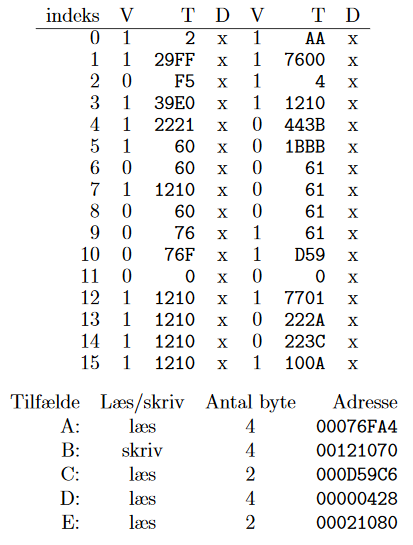
\includegraphics[width=300px]{assets/cacheHistory.png}
			A index 10 no longer valid hit\\
			B index 7 still valid hit\\
			C index 12 miss\\
			D index 2 still valid\\
			E index 8 miss
			
\end{document}
		